%\documentclass[]{slides}
%\title{Computational abstraction}
%
%% Begin document
%\begin{document}
%%\printpdftrue % uncomment to hide pauses
%% Title slide
%\begin{frame} \titlepage \end{frame}
%
%% Outline slide
%%\begin{frame}{Outline} \tableofcontents \end{frame}

% ====================
% Abstraction 
% ====================
\section{Computational abstraction} 
% ====================
% Abstraction Intro
% ====================
\begin{frame}{Computational abstraction}
\begin{itemize}
  \item How would you describe the operation of a computer?
  \item How do users communicate with \acp{IC} inside a computer?
  \pauseprint
  \begin{itemize}
  \item Think about layers.
  \item Between an application (\ac{SW}) and the physics of a computer (\ac{HW}, \acp{IC}, transistors), there are multiple layers that communicate with each other.
  \item Each layer deals with a different complexity level.
  \item Can you name some of these layers?
  \end{itemize}
\end{itemize}
\end{frame}


%% ====================
%% Abstraction HW & SW
%% ====================
%\begin{frame}{Abstraction}
%\begin{figure}
%\centering
%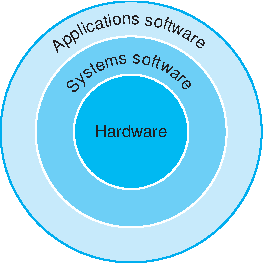
\includegraphics[scale=1]{Abstraction_SW_HW}
%\label{Figure:abstraction_sw_hw}
%\caption{Simplified view of \ac{HW} and \ac{SW} as hierarchical layers.}
%\end{figure}
%\end{frame}

% ====================
% Abstraction HW & SW
% ====================
\begin{frame}{Abstraction}
\vspace{-5pt}
\begin{figure}[!htb]
  \centering
  \begin{minipage}{.49\linewidth}
      \begin{figure}
        \centering
        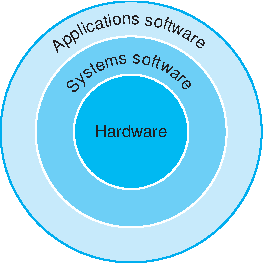
\includegraphics{Abstraction_SW_HW}
        \label{Figure:abstraction_sw_hw}
        \caption{Simplified view of \ac{HW} and \ac{SW} as hierarchical layers.}
      \end{figure}
  \end{minipage}
  \begin{minipage}{.49\linewidth}
      \begin{itemize}
      \item \alertblue{Applications} provide direct user interaction.
      \item \alertblue{System} layer consists of compilers and \acp{OS}.
      \item \alertblue{\ac{HW}} layer relates to the actual physics of the computer, \ie, signals, voltages, shapes, \etc.
      \end{itemize}
  \end{minipage}
\end{figure}
\end{frame}

% ====================
% Abstraction HW & SW
% ====================
\setcounter{figure}{0}
\begin{frame}{Abstraction}
\vspace{-5pt}
\begin{figure}[!htb]
  \centering
  \begin{minipage}{.49\linewidth}
      \begin{figure}
        \centering
        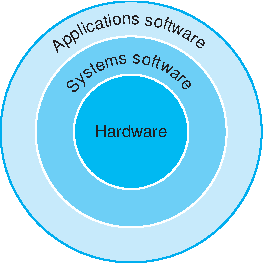
\includegraphics{Abstraction_SW_HW}
        \label{Figure:abstraction_sw_hw}
        %\vspace{-8pt}
        \caption{Simplified view of \ac{HW} and \ac{SW} as hierarchical layers.}
      \end{figure}
  \end{minipage}
  \begin{minipage}{.49\linewidth}
  \alertblue{\ac{OS} basic tasks.}
      \begin{itemize}
        \item Provide interaction between user's programs and the \ac{HW}.
        \item Handling basic \ac{IO} operations.
        \item Allocating storage and memory.
        \item Providing for protected sharing of the computer among multiple applications using it simultaneously.
      \end{itemize}
  \end{minipage}
\end{figure}
\end{frame}

% ====================
% Abstraction HW & SW
% ====================
\begin{frame}{Computational abstraction}
\begin{itemize}
\item Applications such as word processors, internet browsers or media players consists of millions of lines of codes.  
\item \acp{uP} are only capable of executing extremely simple low-level instructions such as additions, comparisons, jumps, load/store from/to memory.
\item Moreover, we must communicate with \ac{HW} by simply using electrical signals.
\pauseprint
\item So how does a computing system perform such complex tasks using limited resources?
\end{itemize}
\end{frame}

% ====================
% Abstraction Gap
% ====================
\begin{frame}{Computational abstraction}
\begin{figure}[!htb]
  \centering
  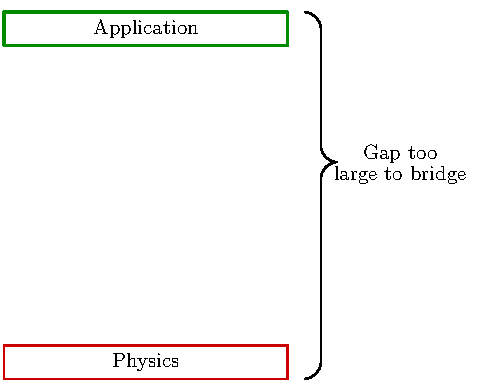
\includegraphics[scale=1]{Abstraction_layers_gap}
  %\caption{Gap.}
  \label{Figure:Abstraction_gap}
\end{figure}
\end{frame}

% ====================
% Abstraction concept
% ====================
\begin{frame}{Computational abstraction}
  \begin{itemize}
  \item \question{How do we fill the gap between the application and the physics?}
  \pauseprint
  \item \answer{The concept of \alert{abstraction}.}
  \pauseprint
  \item Abstraction is no other thing than using different representations of a concept in order to deal with different levels of complexity.
  \item Hiding details when they are not important.
  \item This allows us to focus on a given complexity level and omit unnecessary details.  
  %\item For the example of the NAND2 gate, we can have several representations of this logic gate.
  \end{itemize}
\end{frame}

% ====================
% Abstraction HW & SW
% ====================
\begin{frame}{Computational abstraction}
\begin{itemize}
\item Let's try to bridge the gap starting with the application layer.
\item The application layer is the closest to the user. 
\item Application layer communicates with lower-level layers in order to instruct \ac{HW} what to do.
\item The following elements may be used for this purpose.
\pauseprint
  \begin{itemize}
  \item \alertblue{High-level language.}
  \item \alertblue{Compiler.}
  \item \alertblue{Assembly language.}
  \item \alertblue{Assembler.}
  \item \alertblue{Machine language.}
  \end{itemize}
\end{itemize}
\end{frame}

% ====================
% Abstraction HW & SW
% ====================
\begin{frame}{Computational abstraction}
  \begin{itemize}
  \item \alertblue{High-level language.} \pauseprint Set of words and algebraic notation close to human language used to indicate a sequence of instructions.
  \end{itemize}
  \begin{figure}
    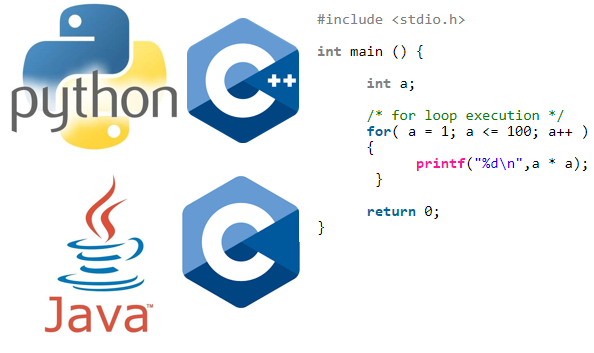
\includegraphics[height=0.6\textheight]{Abstraction_HighLevelLanguagesCode}
  \end{figure}
  \begin{itemize}\pauseprint
  \vspace{-15pt}
    \item \alertblue{Compiler.} \pauseprint Software that translates high-level language to assembly language.
    \end{itemize}
\end{frame}

% ====================
% Abstraction HW & SW
% ====================
\begin{frame}{Computational abstraction}
\vspace{-7pt}
  \begin{itemize}
  \item \alertblue{Assembly language.} Set of words, also called mnemonics or dictionaries, that symbolically represent machine instructions.\pauseprint
  \end{itemize}
  \vspace{-7pt}
  \begin{figure}
    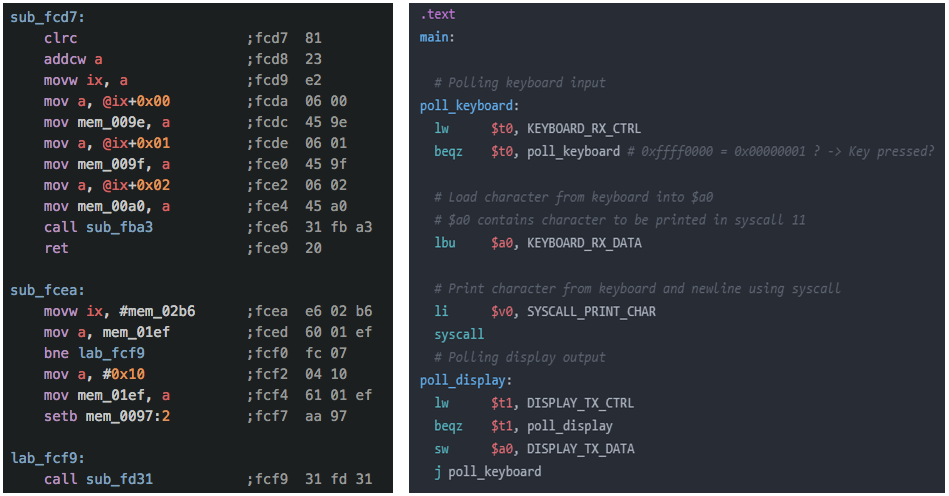
\includegraphics[scale=0.4]{Abstraction_AssemblerCode}
  \end{figure}
  \vspace{-7pt}
  \pauseprint 
  \begin{itemize}
  \item \alertblue{Assembler.} \pauseprint Software that translates assembly language to machine language.\pauseprint
  \item \alertblue{Machine language.} \pauseprint Sequence of bits that represent the most basic operations a machine may perform.
  \end{itemize}
\end{frame}

%% ====================
%% Abstraction HW & SW
%% ====================
%\begin{frame}{Computational abstraction}
%  \begin{itemize}
%  \item \alertblue{High-level language.} \pauseprint Set of words and algebraic notation close to human language used to indicate a sequence of instructions.\pauseprint
%  \item \alertblue{Compiler.} \pauseprint Software that translates high-level language to assembly language.\pauseprint
%  \item \alertblue{Assembly language.} Set of words, also called mnemonics or dictionaries, that symbolically represent machine instructions.\pauseprint
%  \item \alertblue{Assembler.} \pauseprint Software that translates assembly language to machine language.\pauseprint
%  \item \alertblue{Machine language.} \pauseprint Sequence of bits that represent the most basic operations a machine may perform.
%  \end{itemize}
%\end{frame}

% ====================
% Abstraction HW & SW
% ====================
\begin{frame}{Computational abstraction}
\vspace{-5pt}
\begin{figure}[!htb]
  \centering
  \begin{minipage}{.49\linewidth}
      \begin{figure}
        \centering
        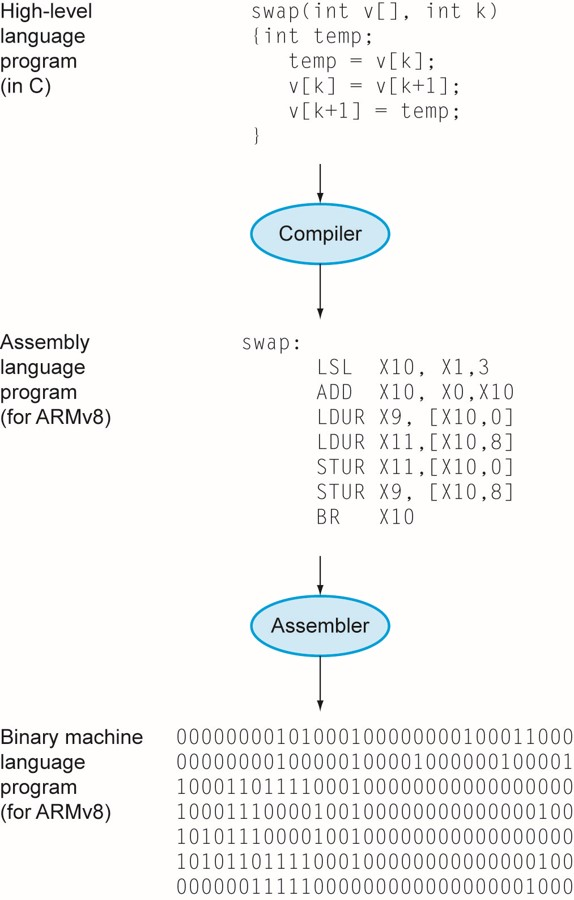
\includegraphics[height=0.75\textheight]{Abstraction_compiler_ARM}
        \label{Figure:abstraction_compiler}
        \vspace{-8pt}
        \caption{High-level language to machine language.}
      \end{figure}
  \end{minipage}
  \begin{minipage}{.49\linewidth}
      \begin{itemize}
      \item The higher the level of the language, the more flexibility it provides.
      \item High-level languages allow programs to be
independent of the computer on which they are developed and deployed.
      \end{itemize}
  \end{minipage}
\end{figure}

\end{frame}

% ====================
% Abstraction Gap
% ====================
\begin{frame}{Computational abstraction}
\begin{figure}[!htb]
  \centering
  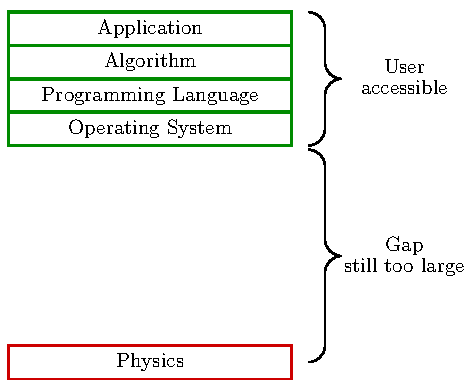
\includegraphics[scale=1]{Abstraction_layers_top}
  %\caption{Gap.}
  \label{Figure:Abstraction_gap_top}
\end{figure}
\end{frame}

% ====================
% Abstraction SV & Layout
% ====================
\begin{frame}{Computational abstraction}
\begin{itemize}
  \item Let's now move to the physical layer.
  \pauseprint
  \item Do these two things represent the same functionality?
\end{itemize}
\begin{figure}[!htb]
  \centering
  \begin{minipage}{.60\linewidth}
      \begin{figure}[!htb]
    \lstset{
        basicstyle=\small,
        xleftmargin=0.05\textwidth, 
        caption=\SV~NAND2 module., 
        label=listing:NAND2
        }
\lstinputlisting{../../../../sv_listings/basic_gates/NAND2.sv}
  \end{figure}

  \end{minipage}
  \begin{minipage}{.35\linewidth}
      \begin{figure}[!htb]
    \centering
    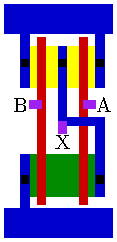
\includegraphics[scale=1.4]{Abstraction_NAND2_layout}
    \caption{NAND2 layout.}
    \label{Figure:NAND2_layout}
  \end{figure}
  \end{minipage}
\end{figure}
\end{frame}

% ====================
% Abstraction Truth table & Schematic
% ====================
\begin{frame}{Computational abstraction}
\begin{itemize}
  \item What about these representations?
  \item Truth table.
  \begin{table}[htb!]
    \centering
      \begin{tabular}{cc||c}
  	    \textbf{A} & \textbf{B} & \textbf{X} \\
  	    \hline
  	    \hline
  	    \code{0} & \code{0} & \code{1} \\ \hline
  	    \code{0} & \code{1} & \code{1} \\ \hline
  	    \code{1} & \code{0} & \code{1} \\ \hline
  	    \code{1} & \code{1} & \code{0} \\ 
  	  \end{tabular}
  \end{table}
  \item Schematic symbol.
  \begin{figure}[!htb]
    \centering
    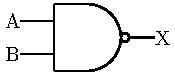
\includegraphics[scale=1]{Abstraction_NAND2}
    \caption{NAND2 gate.}
    \label{Figure:NAND2}
  \end{figure}
\end{itemize}
\end{frame}

% ====================
% Abstraction Transistors & Layout
% ====================
\begin{frame}{Computational abstraction}
\begin{itemize}
  \item What about these representations?
\end{itemize}
\begin{figure}[!htb]
  \centering
  \begin{minipage}{.45\linewidth}
      \begin{figure}[!htb]
    \centering
    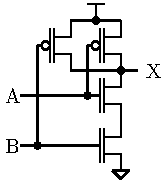
\includegraphics[scale=1.4]{Abstraction_NAND2_transistors}
    \caption{NAND2 transistor level.}
    \label{Figure:NAND2_transistor}
  \end{figure}
  \end{minipage}
  \begin{minipage}{.45\linewidth}
      \begin{figure}[!htb]
    \centering
    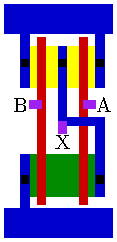
\includegraphics[scale=1.4]{Abstraction_NAND2_layout}
    \caption{NAND2 layout.}
    \label{Figure:NAND2_layout2}
  \end{figure}
  \end{minipage}
\end{figure}
\end{frame}

% ====================
% Abstraction Full
% ====================
\begin{frame}{Computational abstraction}
\begin{figure}[!htb]
  \centering
  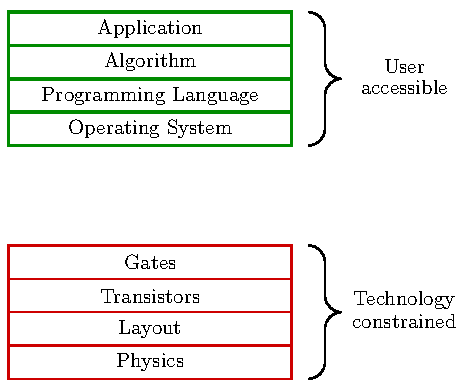
\includegraphics[scale=1]{Abstraction_layers_mid}
  %\caption{Simplified abstraction levels in a computing system.}
  \label{Figure:Abstraction_mid}
\end{figure}
\end{frame}

% ====================
% Abstraction Full
% ====================
\begin{frame}{Computational abstraction}
\begin{itemize}
\item Even with the \alertblue{user} and \alertblue{technology} layers, there is a gap to bridge.
\item \question{How do we fill this gap?}
\pauseprint
\item \answer{Computer Architecture.}
\end{itemize}
\end{frame}

% ====================
% Abstraction Full
% ====================
\begin{frame}{Computational abstraction}
\begin{figure}[!htb]
  \centering
  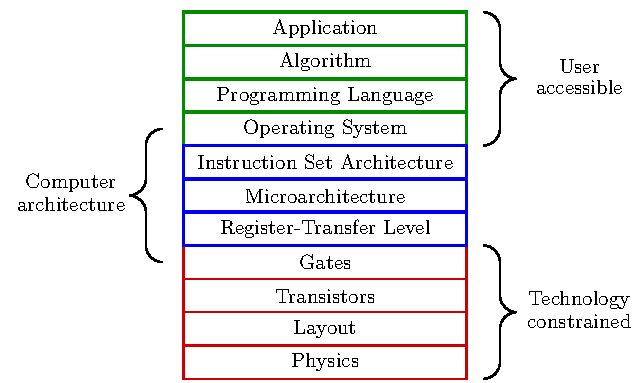
\includegraphics[scale=1]{Abstraction_layers_full}
  \caption{Simplified abstraction levels in a computing system.}
  \label{Figure:Abstraction_full}
\end{figure}
\end{frame}

% ====================
% Abstraction Full
% ====================
\begin{frame}{Computational abstraction}
\begin{itemize}
  \item Computer architecture is the bridge between the user and the physics.
  \item Computer architecture may be seen as the interaction of the basic \ac{HW} building blocks of a computer, as well as the semantics and rules required for such interaction.
  \item The three main components of computer architecture are
    \begin{itemize}
      \item \ac{ISA}.
      \item \ac{uA}.
      \item \ac{RTL}.
    \end{itemize}       
\end{itemize}
\end{frame}

% ====================
% Abstraction Full
% ====================
\begin{frame}{Computational abstraction}
\alertblue{Summary}
\begin{itemize}
\item Abstraction allows us to concentrate on what really matters. 
\item Engineers deal with an abstraction level according to their specialization. For example:
  \begin{itemize}
    \item \ac{SW} engineers do not directly interact with \ac{HW}. However, they must consider some hardware aspects such as memory allocation and usage.
    \item Logic designers may deal with \ac{RTL} and netlist.
    \item Physical design engineers may deal with netlists and layouts.
    \item Layout designers work in routing all the different semiconductor layers in an \ac{IC}.
    \item Analogue designers may work at the transistor and schematic levels.
  \end{itemize}
  \item The higher the abstraction level, the more it may enclose.
  \item Moreover, the concept of abstraction allowed to see where this course is focused on.
\end{itemize}
\end{frame}

%% ====================
%% Abstraction Levels and Design flow
%% ====================
%\begin{frame}{Abstraction and design flow}
%\begin{figure}
%\vspace{-6pt}
%\includegraphics[scale=0.40]{Ychart_radial}
%\vspace{-6pt}
%\caption{Abstraction levels}
%\label{Figure:Ychart_radial}
%\end{figure}
%\end{frame}

%\end{document}
